\documentclass[
	a4paper,
	abstracton,
	emulatestandardclasses
]{scrartcl}

\usepackage[english]{babel}
\usepackage{xcolor}
\usepackage{a4wide}
\usepackage{authblk}
\usepackage{amsthm}
\usepackage{amsmath}
\usepackage{amssymb}
\usepackage{physics}
\usepackage{csquotes}
\usepackage{paralist}
\usepackage[
	backend=biber,
	sorting=none
]{biblatex}
\usepackage{graphicx}
\usepackage{hyperref}
\usepackage{cleveref}
\usepackage[binary-units]{siunitx}
\usepackage[
	margin=10pt,
	labelfont=bf
]{caption}
\usepackage{booktabs}
\usepackage{pgfplots}
\usepackage{adjustbox}
\usepackage[acronym]{glossaries}

\title{MRI to CT Translation with GANs}
\author[1]{Bodo Kaiser}
\author[2]{Shadi Albarqouni}
\affil[1]{\textit{bodo.kaiser@physik.uni-muenchen.de}}
\affil[2]{\textit{shadi.albarqouni@tum.de}}

\DeclareMathOperator{\mae}{MAE}
\DeclareMathOperator{\mse}{MSE}
\DeclareMathOperator{\gdl}{GDL}
\DeclareMathOperator{\psnr}{PSNR}

\pgfplotsset{compat=newest}
\addbibresource{literature.bib}

\glsdisablehyper
\newacronym{ct}{CT}{X-ray computed tomography}
\newacronym{mri}{MRI}{magnetic resonance imaging}
\newacronym{pd}{PD}{proton density}
\newacronym{t1}{T1}{spin-lattice relaxation time}
\newacronym{t2}{T2}{spin-spin relaxation time}
\newacronym{mp}{MP}{magnetization-prepared}
\newacronym{itk}{ITK}{Insight Segmentation and Registration Toolkit}
\newacronym{rage}{RAGE}{RF pulse and rapid gradient echo}
\newacronym{mhd}{MHD}{MetaImage Header}
\newacronym{pet}{PET}{positron emission tomography}
\newacronym{rire}{RIRE}{Retrospective Image Registration Evaluation}
\newacronym{nifti}{NIfTI}{Neuroimaging Informatics Technology Institute}
\newacronym{oasis}{OASIS}{Open Access Series of Imaging Studies}
\newacronym{adni}{ADNI}{Alzheimer's Disease Neuroimaging Initiative}
\newacronym{mae}{MAE}{mean absolute error}
\newacronym{mse}{MSE}{mean squared error}
\newacronym{gan}{GAN}{generative adversarial network}
\newacronym{gdl}{GDL}{gradient distance loss}
\newacronym{psnr}{PSNR}{peak signal-to-noise ratio}

% required to load imshow plots
\newcommand\inputpgf[2]{{
\let\pgfimageWithoutPath\pgfimage
\renewcommand{\pgfimage}[2][]{\pgfimageWithoutPath[##1]{#1/##2}}
\input{#1/#2}
}}

\begin{document}

\makeatletter
\maketitle
\begin{abstract}
  We present a detailed description and reference implementation of
  preprocessing steps necessary to prepare the public \gls{rire} dataset
  for the task of \gls{mri} to \gls{ct} translation. Furthermore we describe
  and implement three state of the art \gls{cnn} and \gls{gan} models where
  we report statistics and visual results of two of them.
\end{abstract}

\makeatother

\section{Introduction}

Computer tomography (CT) and magnetic resonance imaging (MR) are the main
workhorses of clinical diagnosis and cancer monitoring as they reveal the
condition of the patients inner organs.

In consequence of CT and MR exploiting distinct physical effects both
modalities take complementary roles inside the present clinical framework
with MR being more the informative and safe~\cite{Hartwig09} but also
more expensive modality.


While CT is based on the interaction of high energy photons (x-rays) with
biological tissue, MR 


, therefore so called image guided planning based on the
patients CT scan is used to estimate the patients specific radiation treatment
planning. Even though x-rays used for imaging are of a lower energy band
as x-rays used for cancer treatment, it has been shown that they still possess
a risk of developing new cancer inside the patient~\cite{Martin06}.
MR on the other hand takes advantage of the magnetic properties of hydrogen
and is not associated with any health risks . Furthermore MR
provides a much higher soft tissue contrast which is useful for cancer
classification. Although MR and CT differ significant in the applied
physics the high entropy in MR data suggests the existence of a one
directional mapping from MR to CT space whereby the acquisition of CT would
become obsolete. Beside the stated health benefits for the patients such an
approach would reduce expanses and also would free CT resources for
emergency cases where the fast acquisition of CT is used to locate internal
bleedings.

\section{Related Work}

Since the early days of \gls{ct}, health manufacturer were attempted to reduce
radiation exposure in \gls{ct} scans by using, for instance, more sensible
detection electronics, and more sophisticated scanning sequences. Through the
growing availability of computing power we also find evermore computer vision
techniques being utilized, for example, in the enhancement of image quality of
low-dose \gls{ct}s~\cite{Xu12}. Altough these efforts have lead to an
impressive and steady evolution of the \gls{ct} apparatus, they still require
the patient to be irradiated nevertheless.
First approaches which dispense the radiation exposure, through the
computational transformation of \gls{mri} to \gls{ct}, relay on the
atlas-based transformations applied to \gls{mri} to predict \gls{ct}, see
Ref.~\cite{Hofmann08}. Further improvements thereto include, for instance,
random forests~\cite{Andreasen13}. Finally it has been shown that these
\gls{ct} prediction methods can in fact already replace physical \gls{ct}
for treatment planning~\cite{Andreasen2017}.
At the same time, we have seen an incredible progress with deep learning
techniques in computer science~\cite{LeCun15}. Recent efforts with \gls{gan}s,
see Ref.~\cite{Goodfellow14}, seem to be a promising path towards finding
a global optimum in training neural networks through the use of game theory.
Furthermore \gls{gan}s proved significant improvements over the former state
of art in the task of image to image translation~\cite{Isola16} but also the
generalization of three dimensional structures inside the so called latent
space~\cite{ZXFT16}.
Keeping this in mind, the medical computer vision community rapidly adapted
\gls{gan}s for their own specific tasks. In comparison to datasets common in
general computer vision, medical datasets typical comprise volumetric single
channel images with high bit depth. Bearing the challenge of \gls{ct} from
\gls{mri} prediction in mind, the expectations towards \gls{gan}s have been
lately shown increased performance to the previous approaches~\cite{Nie16}.
Yet, the full potential of \gls{gan}s have not been exhausted. For example,
it has been shown that \gls{gan}s are capable of being trained with
unregistered modalities~\cite{Wolterink17}.
Beside the enourmous breakthroughs made in medical computer vision we still
see a shortage in a reproducable comparison of recent methods with publicly
available data. Not to mention the open questions with regard to best
practices in choosing good \gls{gan} model parameters for the task of
\gls{ct} prediction which we hope to address in the subsequent sections.

\section{Method}

In this section we are going to describe the dataset, the performed
preprocessing as well as details on the used neural network models. The
training and prediction was implemented using the Tensorflow library, see
Ref.~\cite{Tensorflow15}.\footnote{The training and prediction scripts are
available at \url{https://github/bodokaiser/mrtoct-tensorflow}.}

\subsection{Dataset}

There are several \gls{mri} and \gls{ct} datasets available, for
instance, \gls{oasis}~\cite{OASIS} or \gls{adni}~\cite{ADNI}. Unfortunately
public datasets in which both modalities are obtainable for the same subject
are, to date, rare. To our knowledge only the \gls{rire} project~\cite{RIRE}
and the Cancer Imaging Archive~\cite{CIA} provide \gls{mri} and \gls{ct}
volumes for some subjects. For the present work we limited ourselves to the
data from the \gls{rire} project, as the volumetric data was available in the
same format.
\begin{table}[h]
  \centering
  \begin{tabular}{*{6}{c}}
    \toprule
    & \multicolumn{4}{c}{\acrshort{mri}}
		& \\
   	\cmidrule{2-5}
    \acrshort{ct} &
		\acrshort{pd} &
		\acrshort{t1} &
		\acrshort{t2} &
		\acrshort{mp} \acrshort{rage} &
		\acrshort{pet} \\
    \midrule
    \num{17} & \num{14} & \num{19} & \num{18} & \num{9} & \num{8} \\
             & \num{12} & \num{17} & \num{16} & \num{9} & \num{6} \\
    \bottomrule
  \end{tabular}
  \caption{Subject statistics with respect of the available imaging
    modalities of the \gls{rire} dataset. The second table only accounts for
    subjects with available \gls{ct} data.
  }\label{tab:rire}
\end{table}
In \Cref{tab:rire} we list the aggregated modality count of the \gls{rire}
dataset (first row). As we use the \gls{ct} as target space, we created a
second modality count on the subjects with \gls{ct} modality (second row).
Beside of \gls{ct} one can also obtain \gls{pet} images for some subjects.
Next to the common \gls{t1} and \gls{t2} weighted \gls{mri}, some subjects of
the \gls{rire} dataset also offer \gls{pd} and \gls{mp} \gls{rage} weighted
\gls{mri}s. Some \gls{mri}s can be obtained in a rectified version, which we
did not use. We used the \gls{t1} weighted \gls{mri} together with the
\gls{ct} as input and target data as these give us the highest subject count.
However, it would be an interesting experiment to supply different \gls{mri}s
as multi-channel input.

\subsection{Preprocessing}

The modality data for each subject can be downloaded from the website of the
\gls{rire} project, see Ref.~\cite{RIRE}. In \Cref{fig:conversion} we depicted
the first preprocessing step, that involves the extraction, decompression and
conversion of the downloaded data. After extraction and decompression the
volumetric data presents itself as \gls{mhd}. We converted the \gls{mhd} files
to the self-contained \gls{nifti} format through the Python front-end of the
\gls{itk} library.
\begin{figure}[h]
  \centering
  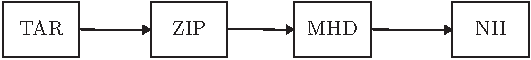
\includegraphics[page=1,width=\linewidth]{figure/diagrams.pdf}
  \caption{Image extraction and conversion from \gls{mhd} to \gls{nifti}
		format.
	}\label{fig:conversion}
\end{figure}
\Cref{fig:registration} illustrates the coregistration procedure as part of
the image preprocessing. The coregistration yields a rigid transformation that
aligns the moving volume with the fixed volume. In our case it makes sense to
use the \gls{ct} volume as the fixed volume because the \gls{ct} are in
general better centered. Given a rigid transformation, a linear interpolator
returns a translated volume from the sample points of the initial \gls{mri}.
The mutual information between the moved \gls{mri} and the \gls{ct} is then
used to optimize the rigid transformation. The procedure is executed
iteratively and stopped when the maximum iterations steps are reached or
the convergence parameter is met. As the implementation of the interpolator
and transformation optimizer is not a trivial undergoing, therefore we
reverted back to the \gls{itk} library, see Ref.~\cite{Yaniv2018}.
\begin{figure}[h]
  \centering
  \includegraphics[page=2,width=\linewidth]{figure/diagrams.pdf}
  \caption{Multi-modal image coregistration using maximum mutual information
    optimizer.
	}\label{fig:registration}
\end{figure}
Following the coregistration, we used the binary fill holes algorithm from
SciPy~\cite{SciPy} to remove the \gls{ct} table present in some \gls{ct}
volumes as well as well as background noise.\footnote{The complete
preprocessing described so far is available at
\url{https://github/bodokaiser/mrtoct-scripts}.} Finally we converted the
preprocessed pairs of \gls{mri} and \gls{ct} volumes to the tfrecord format
in order to easily read the data into Tensorflow~\cite{Tensorflow15}. As part
of the data pipeline implemented with Tensorflow we do a pad or crop to either
$384\times384$ for transverse 2D slices or $32\times32\times32$ for \gls{mri}
respective $16\times16\times16$ for \gls{ct} for 3D patches. The target shape
for the 2D slices was choosen to be compatible with the convolution parameters
and the largest resolution of all volumes. Furtheremore we applied a
min-max-normalization in order to operate on a value range of $[0,1]$.

\subsection{Models}

We implemented three different neural network models for the \gls{mri} to
\gls{ct} synthesis task. The first and most simple model is based on the
u-net model~\cite{Ronneberger15} and uses standard metric error metric,
i.e.\ \gls{mae} and \gls{mse}. The second model is based on
pix2pix~\cite{Isola16}, which already has proven great success in the task
of image translation. It uses the first u-net based model as generator in
addition to a discriminator model to calculate the adversarial loss. As third
model we implemented the context-aware 3D synthesis GAN from Nie~\cite{Nie16}.
In comparison to the other two models, which operate on the transverse 2D
slices of the brain, it is applied to 3D patches.

\subsubsection{u-net}

The original u-net model~\cite{Ronneberger15} was developed for the
segmentation of biomedical images. The key idea of the architecture is to
combine the capture of context and precise localization through interconnected
layers.
\begin{figure}[h]
  \centering
  \includegraphics[page=3,width=\linewidth]{figure/diagrams.pdf}
  \caption{The u-net generator architecture.
  }\label{fig:unet:gen}
\end{figure}
In \Cref{fig:unet:gen} the u-net architecture is illustrated. The
input \gls{mri} slice is of shape $384\times384\times1$, wherein the last
dimension corresponds to the number of channels. In case one would like to
input different weighted \gls{mri}s, it would be possible to concat these into
the last dimension as long as they are properly coregistered.
We can see that there are two paths of data flow: for one the image is passed
through a seqeunce of encoders and decoders, then again data can flow from
one encoder stage directly to the symmetric decoder stage. The encoder decode
features with increasing coarse resolution, while the decoders synthesize the
target image from the previous stage and the feature map of same resolution.
\begin{figure}[h]
  \centering
  \includegraphics[page=4,width=\linewidth]{figure/diagrams.pdf}
  \caption{The u-net encoder, decoder and final convolution block.
	}\label{fig:unet:blocks}
\end{figure}
In \Cref{fig:unet:blocks} we present the exact layer composition of the
encoder, decoder and final block of the u-net architecture. In comparison to
the original u-net we reduced the convolution layers per block to one and
replaced the max-pooling in the decoders with deconvolutions. Furthermore
we used Leaky ReLUs in the encoders. These changes are mainly inspired by the
u-net like generator used in pixtopix. The first encoder block uses no batch
normalization and dropout is only used in Decoder \num{4} and Decoder \num{5}
as noted in \Cref{fig:unet:gen}.
\begin{table}[h]
  \centering
  \begin{tabular}{lcccc}
    \toprule
    Block & Kernel & Strides & Padding & Initializer \\
    \midrule
    Encode & \num{4} & \num{2} & Same & Xavier \\
    Decode & \num{4} & \num{2} & Same & Xavier \\
    Final  & \num{3} & \num{2} & Same & Xavier \\
    \bottomrule
  \end{tabular}
  \caption{Convolution parameters used in the u-net blocks.
  }\label{tab:unet:conv}
\end{table}
In \Cref{tab:unet:conv} the convolution parameters for the convolution and
deconvolution layers in the u-net blocks are shown. The kernel paremeter
specifies the size of the convolution kernel, the stride parameter describes
the spacing in between applied convolutions. The padding algorithm was chosen
to keep output and input size the same. Weight initialization was performed
according using Xavier, see Ref.~\cite{Xavier2010}.

\subsubsection{pixtopix}

The pixtopix model uses the previously described u-net as generator in
addition to a discriminator to supply an adversarial score, see
Ref.~\cite{Isola16}. It has proven great success as general purpose solution
for translation experiments with color images. Recently the pixtopix was
extended to support training on unpaired data~\cite{Zhu2017}. This approach
has also already been applied successfully to the task of \gls{mri} to
\gls{ct} translation~\cite{Wolterink17}.
\begin{figure}[h]
  \centering
  \includegraphics[page=5,width=\linewidth]{figure/diagrams.pdf}
  \caption{The pixtopix discriminator architecture.
	}\label{fig:pixtopix:disc}
\end{figure}
In \Cref{fig:pixtopix:disc} the discriminator architecture is depicted. It
first concats the input \gls{mri} with either the target \gls{ct} or the
output \gls{ct}, depending on if we want to calculate a real or fake score,
in the channel dimension. The image of shape $384\times384\times2$ is then
passed through five convolutional layer that finally output a score map of
shape $1\times24\times512$.
\begin{figure}[h]
  \centering
  \includegraphics[page=6,width=\linewidth]{figure/diagrams.pdf}
  \caption{The pixtopix discriminator blocks.
	}\label{fig:pixtopix:blocks}
\end{figure}
In \Cref{fig:pixtopix:blocks} we see that the convolutional blocks comprise
a convolutional layer and a Leaky ReLU non-linearity, wherein the final block
uses a Sigmoid activation instead of Leaky ReLUs.
\begin{table}[h]
  \centering
  \begin{tabular}{lcccc}
    \toprule
    Block & Kernel & Strides & Padding & Initializer \\
    \midrule
    Conv & \num{4} & \num{2} & Same & Xavier \\
    Final  & \num{4} & \num{1} & Same & Xavier \\
    \bottomrule
  \end{tabular}
  \caption{Convolution parameters used in the pixtopix discriminator blocks.
  }\label{tab:pixtopix:conv}
\end{table}
\Cref{tab:pixtopix:conv} shows the exact configuration of the convolutional
layers in the pixtopix discriminator blocks.

\subsubsection{Context-aware 3D synthesis}

The last model uses 3D patches of shape $32\times32\times32$ from the
\gls{mri} to synthesize \gls{ct} patches of shape $16\times16\times16$. By
using a larger volume for the input the network is able to perform
context-aware synthesis. Furthermore the patch-based data approach allows the
support of different sized brain volumes or even only specific subregions ---
as long as the voxel size correspond to the same world sizes --- which is
useful for practical applications. Unfortunately this approach puts a lot
complexity in the pre- and postprocessing, as we need to extract the patches
first from the volume and then need to recombine them at a later stage.
\begin{figure}[h]
  \centering
  \includegraphics[page=7,width=\linewidth]{figure/diagrams.pdf}
  \caption{The contxt-aware 3D synthesis generator architecture.
  }\label{fig:synthesis:gen}
\end{figure}
\begin{figure}[h]
  \centering
  \includegraphics[page=8,width=\linewidth]{figure/diagrams.pdf}
  \caption{The context-aware 3D synthesis discriminator architecture.
	}\label{fig:synthesis:disc}
\end{figure}
In \Cref{fig:synthesis:gen} and \Cref{fig:synthesis:disc} we illustrated the
generator and discriminator architecture of the context-aware 3D synthesis
model. The generator iteratively convolves the input \gls{mri} patch to the
target \gls{ct} patch. In comparison to the u-net based generators there
are no interconnected layers. The discriminator takes a similar approach and
reduces the output or target \gls{ct} patch to a score map of shape
$8\times8\times8\times1$. In comparison to pixtopix it does not consider the
input \gls{mri}.
\begin{figure}[h]
  \centering
  \includegraphics[page=9,width=\linewidth]{figure/diagrams.pdf}
  \caption{The context-aware 3D synthesis generator and discriminator dense
    and convolution blocks.
	}\label{fig:synthesis:blocks}
\end{figure}
In \Cref{fig:synthesis:blocks} we see the internal structure of the
convolution blocks in both the generator and the discriminator. In comparison
to pixtopix it uses normal ReLUs and max pooling over deconvolution.
\begin{table}[h]
  \centering
  \begin{tabular}{lccc}
    \toprule
    Block         & Kernel  & Padding & Filters \\
    \midrule
    Gen. Conv 1   & \num{9} & Valid   & 32      \\
    Gen. Conv 2   & \num{3} & Same    & 32      \\
    Gen. Conv 3   & \num{3} & Valid   & 32      \\
    Gen. Conv 4   & \num{3} & Valid   & 32      \\
    Gen. Conv 5   & \num{9} & Same    & 64      \\
    Gen. Conv 6   & \num{3} & Valid   & 64      \\
    Gen. Conv 7   & \num{3} & Valid   & 32      \\
    Gen. Conv 8   & \num{7} & Valid   & 32      \\
    Gen. Conv 9   & \num{3} & Valid   & 32      \\
    Gen. Conv 10  & \num{3} & Valid   & 1       \\
    Disc. Conv 1  & \num{5} & Same    & 32      \\
    Disc. Conv 2  & \num{5} & Same    & 64      \\
    Disc. Conv 3  & \num{5} & Same    & 128     \\
    Disc. Conv 4  & \num{5} & Same    & 256     \\
    \bottomrule
  \end{tabular}
  \caption{Convolution parameters used in the context-aware 3D synthesis
    blocks. Strides default to \num{1}. Weight initialization was performed
    through Xavier.
  }\label{tab:synthesis:conv}
\end{table}
\Cref{tab:synthesis:blocks} discloses the convolution parameters used. Though
the kernel size was given in Ref.~\cite{Nie16}, we had to experiment with
the padding and the stride parameter in order to get the dimension reduction
to $16\times16\times\16$.
\begin{figure}[h]
  \centering
  \includegraphics[page=10,width=\linewidth]{figure/diagrams.pdf}
  \caption{The auto-context model used in ontext-aware 3D synthesis for
    image refinement.
	}\label{fig:synthesis:refine}
\end{figure}
We already noted that the context-aware 3D synthesis generator lacks
interconnected layers in comparison to u-net. Instead, it uses the
auto-context model first introduced in Ref.~\cite{Tu2010}. The concept is
illustrated in \Cref{fig:synthesis:refine}. The idea is to iteratively train
networks and to pass the previous results with the initial \gls{mri} to the
preceeding stage.

\section{Experiments}

We had difficulties with the implementation of the patch aggregation required
for the implementation of the context-aware 3D synthesis. Though patch
aggregation worked in general, it occupied more computational resources than
the actual training. Unfortunatly we were not able to find a workaround or to
allocate more computation quota. Therefor we did not perform more than one
iteration of the auto-context model, which prevented a fair comparison.
However, we encourage everyone to test our implementation themselves.
As a consequence we only conducted experiments with the u-net generator and
the pixtopix \gls{gan}.

\subsection{Distance Losses}

One experimental parameter of interest was the performance impact of the
different loss functions. We first optimized the loss function used when
only training the u-net. Let $X,Y\in{[0,1]}^N$ be output and target vectors,
then we define the \gls{mae} to be
\begin{equation}
  \mae\left(X,Y\right)
  =
  \frac{1}{N}\sum_{i=1}^N
  \abs{X_i-Y_i}
  \label{eq:mae}.
\end{equation}
The \gls{mse} we define via
\begin{equation}
  \mse\left(X,Y\right)
  =
  \frac{1}{N}\sum_{i=1}^N
  {\left(X_i-Y_j\right)}^2
  \label{eq:mse}.
\end{equation}
Finally the \gls{gdl} disclosed in Ref.~\cite{Nie16} is defined as
\begin{equation}
  \gdl\left(X,Y\right)
  =
  \mse\left(\grad X,\grad Y\right)
  \label{eq:gdl},
\end{equation}
wherein $\grad$ is the spatial gradient. We approximate the $i$th element
of the spatial gradient through
\begin{equation}
  \grad X_i
  \approx
  \begin{cases}
    X_i-X_{i+1}\qc\text{if }, $1<i<N$\\
    0\qc\text{otherwise}
  \end{cases}
  \label{eq:grad}.
\end{equation}
The loss terms can of course be combined
\begin{equation}
  \lambda_\text{MAE}\mae\left(X,Y\right)
  +
  \lambda_\text{MSE}\mse\left(X,Y\right)
  +
  \lambda_\text{GDL}\gdl\left(X,Y\right),
\end{equation}
wherein the $\lambda$ denotes the weight of the respective loss term.

\begin{table}[h]
  \centering
  \begin{tabular}{ccc}
    \toprule
    Dataset & Subject & Shape \\
    \midrule
    Training & \num{1} & \num{161x320x250x1} \\
    Training & \num{2} & \num{149x328x250x1} \\
    Training & \num{3} & \num{112x303x281x1} \\
    Training & \num{4} & \num{155x291x259x1} \\
    Training & \num{5} & \num{143x307x284x1} \\
    Training & \num{6} & \num{149x278x267x1} \\
    Training & \num{7} & \num{200x289x268x1} \\
    Training & \num{8} & \num{218x282x238x1} \\
    Training & \num{9} & \num{191x322x252x1} \\
    Training & \num{10} & \num{200x303x243x1} \\
    Training & \num{11} & \num{181x317x239x1} \\
    Training & \num{12} & \num{186x310x248x1} \\
    Training & \num{13} & \num{112x313x238x1} \\
    Validation & \num{1} & \num{112x298x227x1} \\
    Validation & \num{2} & \num{223x328x282x1} \\
    Validation & \num{3} & \num{223x307x276x1} \\
    Validation & \num{4} & \num{204x329x262x1} \\
    \bottomrule
  \end{tabular}
  \caption{Training and validation dataset volumes used in this section. The
    dimensions of the shape correspond to depth, height and width.
  }\label{tab:unet:dataset}
\end{table}

\begin{table}[h]
  \centering
  \begin{tabular}{cccccc}
    \toprule
    & &
    \multicolumn{2}{c}{\acrshort{mae}} &
    \multicolumn{2}{c}{\acrshort{mae}+\acrshort{gdl}} \\
    Image Slices & Batch Size & Steps & Epochs & Steps & Epochs \\
    \midrule
    \num{2157} & \num{16} & \num{20542} & \num{152} & \num{19388} & \num{143} \\
    \bottomrule
  \end{tabular}
  \caption{Training parameters used for the distance metrics experiments.
  }\label{tab:unet:params}
\end{table}

\begin{table}[h]
  \centering
  \begin{tabular}{ccccc}
    \toprule
    $\lambda_\text{mae}$ &
    $\lambda_\text{gdl}$ &
    \acrshort{mae} &
    \acrshort{mse} &
    \acrshort{psnr} \\
    \midrule
    \num{1} & \num{0} & \num{31.58} & \num{6577} & \num{59.5} \\
    \num{1} & \num{1e-7} & \num{37.15} & \num{7945} & \num{58.1} \\
    \bottomrule
  \end{tabular}
  \caption{Distance metrics for the u-net model trained with different loss
    functions, evaluated on the training dataset.
  }\label{tab:unet:training}
\end{table}
\begin{table}[h]
  \centering
  \begin{tabular}{ccccc}
    \toprule
    $\lambda_\text{mae}$ &
    $\lambda_\text{gdl}$ &
    \acrshort{mae} &
    \acrshort{mse} &
    \acrshort{psnr} \\
    \midrule
    \num{1} & \num{0} & \num{123.6} & \num{70846} & \num{47.93} \\
    \num{1} & \num{1e-7} & \num{129.0} & \num{72704} & \num{47.90} \\
    \bottomrule
  \end{tabular}
  \caption{Distance metrics for the u-net model trained with different loss
    functions, evaluated on the validation dataset.
  }\label{tab:unet:validation}
\end{table}
\begin{figure}[h]
  \centering
  \begin{adjustbox}{width=\linewidth}
    \inputpgf{figure}{unet-training.pgf}
  \end{adjustbox}
  \caption{Transverse views for the u-net model trained with different
    loss functions, evaluated on the training dataset.
  }\label{fig:unet:training}
\end{figure}
\begin{figure}[h]
  \centering
  \begin{adjustbox}{width=\linewidth}
    \inputpgf{figure}{unet-validation.pgf}
  \end{adjustbox}
  \caption{Transverse views for the u-net model trained with different
    loss functions, evaluated on the validation dataset.
  }\label{fig:unet:validation}
\end{figure}

\subsection{Adversarial Losses}

\begin{table}[h]
  \centering
  \begin{tabular}{ccc}
    \toprule
    Dataset & Subject & Shape \\
    \midrule
    Training & \num{1} & \num{137x320x250x1} \\
    Training & \num{2} & \num{130x328x250x1} \\
    Training & \num{3} & \num{111x303x281x1} \\
    Training & \num{4} & \num{143x291x259x1} \\
    Training & \num{5} & \num{141x307x284x1} \\
    Training & \num{6} & \num{148x278x267x1} \\
    Training & \num{7} & \num{198x289x268x1} \\
    Training & \num{8} & \num{208x282x238x1} \\
    Training & \num{9} & \num{162x322x252x1} \\
    Training & \num{10} & \num{185x303x243x1} \\
    Training & \num{11} & \num{180x317x239x1} \\
    Training & \num{12} & \num{184x310x248x1} \\
    Training & \num{13} & \num{93x313x238x1} \\
    Validation & \num{1} & \num{105x298x227x1} \\
    Validation & \num{2} & \num{190x328x282x1} \\
    Validation & \num{3} & \num{202x307x276x1} \\
    Validation & \num{4} & \num{198x329x262x1} \\
    \bottomrule
  \end{tabular}
  \caption{Training and validation dataset volumes used in this section. The
    dimensions of the shape correspond to depth, height and width.
  }\label{tab:unet_pixtopix:dataset}
\end{table}

\begin{table}[h]
  \centering
  \begin{tabular}{cccccc}
    \toprule
    & &
    \multicolumn{2}{c}{u-net (\gls{mae})} &
    \multicolumn{2}{c}{pixtopix} \\
    Image Slices & Batch Size & Steps & Epochs & Steps & Epochs \\
    \midrule
    \num{2020} & \num{16} & \num{22080} & \num{174} & \num{37832} & \num{299} \\
    \bottomrule
  \end{tabular}
  \caption{Training parameters used for the u-net and pixtopix comparison.
  }\label{tab:unet_pixtopix:params}
\end{table}
\begin{table}[h]
  \centering
  \begin{tabular}{ccccc}
    \toprule
    Model & Loss &
    \acrshort{mae} &
    \acrshort{mse} &
    \acrshort{psnr} \\
    \midrule
    u-net & \acrshort{mae} & \num{90.5} & \num{61853} & \num{49.4} \\
    pixtopix & least-square & \num{21.6} & \num{4210} & \num{60.4} \\
    \bottomrule
  \end{tabular}
  \caption{Distance metrics for the u-net model trained with \acrshort{mae}
    loss compared with the pixtopix model trained with least-square adversarial
    loss, evaluated on the training dataset.
  }\label{tab:unet_pixtopix:training}
\end{table}
\begin{table}[h]
  \centering
  \begin{tabular}{ccccc}
    \toprule
    Model & Loss &
    \acrshort{mae} &
    \acrshort{mse} &
    \acrshort{psnr} \\
    \midrule
    u-net & \acrshort{mae} & \num{136.9} & \num{101943} & \num{46.77} \\
    pixtopix & least-square & \num{112.7} & \num{82173} & \num{47.55} \\
    \bottomrule
  \end{tabular}
  \caption{Distance metrics for the u-net model trained with \acrshort{mae}
    loss compared with the pixtopix model trained with least-square adversarial
    loss, evaluated on the validation dataset.
  }\label{tab:unet_pixtopix:training}
\end{table}
\begin{figure}[h]
  \centering
  \begin{adjustbox}{width=\linewidth}
    \inputpgf{figure}{unet-pixtopix-training.pgf}
  \end{adjustbox}
  \caption{Transverse views for the u-net model trained with \acrshort{mae}
    loss compared with the pixtopix model trained with least-square adversarial
    loss, evaluated on the training dataset.
  }\label{fig:unet_pixtopix:training}
\end{figure}
\begin{figure}[h]
  \centering
  \begin{adjustbox}{width=\linewidth}
    \inputpgf{figure}{unet-pixtopix-validation.pgf}
  \end{adjustbox}
  \caption{Transverse views for the u-net model trained with \acrshort{mae}
    loss compared with the pixtopix model trained with least-square adversarial
    loss, evaluated on the validation dataset.
  }\label{fig:unet_pixtopix:validation}
\end{figure}

\subsection{Gradient Boost}

\begin{table}[h]
  \centering
  \begin{tabular}{cccccc}
    \toprule
    & &
    \multicolumn{2}{c}{u-net (\gls{mae})} &
    \multicolumn{2}{c}{pixtopix} \\
    Image Slices & Batch Size & Steps & Epochs & Steps & Epochs \\
    \midrule
    \num{2020} & \num{16} & \num{37832} & \num{299} & \num{51911} & \num{411} \\
    \bottomrule
  \end{tabular}
  \caption{Training parameters used for pixtopix and gradient boosted
    fine-tuned pixtopix model.
  }\label{tab:pixtopix:params}
\end{table}
\begin{table}[h]
  \centering
  \begin{tabular}{ccccc}
    \toprule
    Model & Loss &
    \acrshort{mae} &
    \acrshort{mse} &
    \acrshort{psnr} \\
    \midrule
    pixtopix & least-square & \num{21.56} & \num{4210} & \num{60.38} \\
    pixtopix (boosted) & least-square & \num{23.37} & \num{4140} & \num{60.30} \\
    \bottomrule
  \end{tabular}
  \caption{Distance metrics for the pixtopix model trained with least-square
    adversarial loss compared to fine-tuned with gradient boost, evaluated on
    the training dataset.
  }\label{tab:pixtopix:training}
\end{table}
\begin{table}[h]
  \centering
  \begin{tabular}{ccccc}
    \toprule
    Model & Loss &
    \acrshort{mae} &
    \acrshort{mse} &
    \acrshort{psnr} \\
    \midrule
    pixtopix & least-square & \num{112.73} & \num{82173} & \num{47.55} \\
    pixtopix & least-square & \num{112.23} & \num{79296} & \num{47.68} \\
    \bottomrule
  \end{tabular}
  \caption{Distance metrics for the pixtopix model trained with least-square
    adversarial loss compared to fine-tuned with gradient boost, evaluated on
    the validation dataset.
  }\label{tab:pixtopix:validation}
\end{table}
\begin{figure}[h]
  \centering
  \begin{adjustbox}{width=\linewidth}
    \inputpgf{figure}{pixtopix-training.pgf}
  \end{adjustbox}
  \caption{Transverse views for the pixtopix model trained with least-square
    adversarial loss compared to fine-tuned with gradient boost, evaluated on
    the validation dataset.
  }\label{fig:pixtopix:training}
\end{figure}
\begin{figure}[h]
  \centering
  \begin{adjustbox}{width=\linewidth}
    \inputpgf{figure}{pixtopix-validation.pgf}
  \end{adjustbox}
  \caption{Transverse views for the pixtopix model trained with least-square
    adversarial loss compared to fine-tuned with gradient boost, evaluated on
    the validation dataset.
  }\label{fig:pixtopix:validation}
\end{figure}



\clearpage
\printbibliography{}

\end{document}
